\lecture{1}{From Thermodynamics to Statistics}{Qiang Zhu}{scribe-name1,2,3}

\section{An overview about thermodynamics} % Don't be this informal in your notes!
Thermodynamics is aimed at describing the macroscopic phenomenon such as heat transfer, energy conversion, chemical reactions.
We study them by measuring some key quantities (such as pressure, temperature, volume, viscosity, bulk modulus, .etc) and their correlations.
The foundation of thermodynamics is based on the thermodynamic laws:
\begin{enumerate}
	\item energy cannot be created or destroyed in an isolated system.
	\item the entropy of any isolated system always increases
	\item the entropy of a system approaches a constant value as the temperature approaches absolute zero
\end{enumerate}	

We can understand the general picture by studying the following equations
\begin{equation} \label{idealgas} PV = nRT = NkT \end{equation}
\begin{equation} \label{Avogadro} N = n \times N_A \end{equation}
%\begin{equation} \label{PV-micro} PV = Nm{\overline v_x^2} = NkT\end{equation}
\begin{equation} \label{eqpartition} U_{thermal} = N \cdot f \cdot \frac{1}{2}kT \end{equation}
\begin{equation} \label{1stlaw} \Delta{U} = Q + W \end{equation}
\begin{equation} \label{work3} \Delta W = - P \Delta{V} \end{equation}
\begin{equation} \label{entropy} S = k \text{ln}\Omega \end{equation}
\begin{equation} dU = TdS - PdV  + \mu dN\end{equation}

However, thermodynamics does not tell us the microscopic details about the matter. We observe heat always flows spontaneously from a hot object to a cold one. The underlying explanation of this thermodynamic phenomenon is due to the change of entropy, a microscopic phenomenon. We might briefly discussed them to some extents in thermodynamic classes. Here, we are going to to explore them more comprehensively with the tool of statistic mechanics.

\section{Kinetic Theory of Gases}
\begin{figure}[h]
\centering
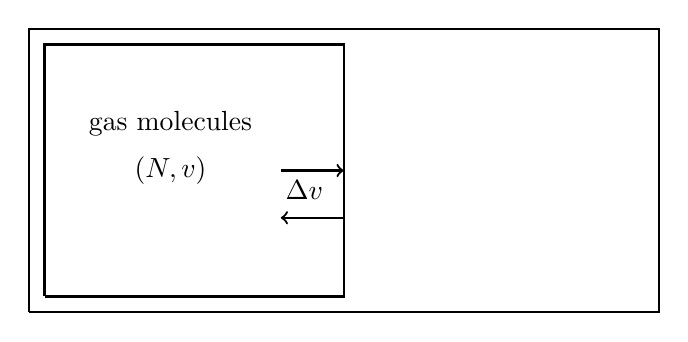
\begin{tikzpicture}[thick]
\draw (0,0.4) -- (8,0.4) -- (8,4) -- (0,4) -- (0,0.4);
\draw (0.2,0.6) -- (4.0,0.6) -- (4.0,3.8) -- (0.2,3.8) -- (0.2,0.6);
\node at (1.8,2.8) {gas molecules};
\node at (1.8,2.2) {($N, v$)};
	\draw [->] (3.2,2.2) -- (4.0,2.2) node [below, xshift=-0.5cm]{$\Delta{v}$};
	\draw [->] (4.0,1.6) -- (3.2,1.6);
\end{tikzpicture}
\caption{A schematic of gases in a container.}
\end{figure}

In the early days of thermal physics, it was primarily shaped by experimental studies of the macroscopic behavior of physical systems, through the work of Carnot, Joule, Clausius and Kelvin. However, people were keen to know how the observed phenomenon were related to the motion of molecules and atoms.

The first attempt was the so called kinetic theory of gases, which aimed at explaining the macroscopic behavior of gaseous systems in terms of the motion of molecules. Although a bit speculative, it began to emerge as a real mathematical theory. 

The theory for ideal gases makes the following assumptions:
\begin{enumerate}
	\item The gas consists of very small particles known as molecules separate by large distances
	\item The number of molecules is so large that statistical treatment can be applied.
	\item These molecules are in constant, random, and rapid motion.
	\item The rapidly moving particles constantly collide among themselves and with the walls of the container. 
	\item All these collisions are perfectly elastic. 
	\item Except during collisions, the interactions among molecules are negligible. 
\end{enumerate}	
With these assumptions, we then proceed to figure the relations between the pressure and atomic motion. In such model, the pressure is equal to the force exerted by the atoms hitting and rebounding from a unit area of wall. Consider a gas of $N$ molecules, each of mass $m$, enclosed in a cube with $V = L^3$. When a gas molecule collides with the wall perpendicular to the x axis and bounces off in the opposite direction with the same speed (an elastic collision), the change in momentum is given by:


\begin{equation} \Delta P = p_{i,x} - p_{f,x} = m(v_x) - m(-v_x) = 2mv_x \end{equation}
where $p$ is the momentum, $i$ and $f$ indicate the initial and final state, v is the speed of particle.
The particle impacts once wall once every
\begin{equation} \Delta t = \frac{2L}{v_x} \end{equation}
where $L$ is the distance between two walls.
The force contributed from one particle can be expressed as 
\begin{equation} F = \frac{\Delta p}{\Delta t} = \frac{mv_x^2}{L}\end{equation}
Since we have many particles, the total force on the wall is:
\begin{equation} F = \frac{m\bar{v_x^2}}{L}\end{equation}

Since the motion of the particles is random and there is no bias applied to any direction, the averaged speed in each direction should be identical.
\begin{equation} \bar{v_x^2} = \bar{v_y^2} = \bar{v_z^2}  \end{equation}
\begin{equation} \bar{v^2} = \bar{v_x^2} + \bar{v_y^2} + \bar{v_z^2} = 3\bar{v_x^2} \end{equation}

And the force is
\begin{equation} F = \frac{Nm\bar{v^2}}{2L} \end{equation}
So we obtain the pressure
\begin{equation} P = \frac{F}{L^2} = \frac{Nm\bar{v^2}}{3V} \end{equation}

In term of the kinetic energy ($K=1/2Nm\bar{v^2}$),
\begin{equation} PV = \frac{2K}{3} \end{equation}

This is a first non-trivial result of the kinetic theory because it relates pressure (a macroscopic property), to the (translational) kinetic energy of the molecules (a microscopic property).

From the ideal gas law $PV=nRT=NkT$, we can further derive the relation between $K$ and $T$.

\begin{equation} PV = \frac{2K}{3} = NkT \end{equation}

As one can see, this simple scheme could successfully explain some key features in an elegant way. 
However, it is limited by the oversimplified assumptions.
The real contact with thermodynamics could not be made until 1872 when Boltzmann developed his $H$-theorem and established a direct connection between entropy and molecular dynamics. 
Simultaneously, the kinetic theory began giving away to its more sophisticated successor - the ensemble theory.
The power of the techniques that finally emerged reduced thermodynamics to the status of an consequence of the statistics and the mechanics of the molecules constituting a given physical system.
It was then natural to give the formalism name $Statistical Mechanics$

%\end{document}

